%& -shell-escape
%%% Copyright (c) 2011, Илья w-495 Никитин
%%%
%%% Разрешается повторное распространение и использование как в виде исходного
%%% кода, так и в двоичной форме, если таковая будет получена, 
%%% с изменениями или без, при соблюдении следующих условий:
%%%
%%%     * При повторном распространении исходного кода должно оставаться
%%%       указанное выше уведомление об авторском праве, этот список условий и
%%%       последующий отказ от гарантий.
%%%     * Ни имя w-495, ни имена друзей или консультантов не могут быть
%%%       использованы в качестве поддержки или продвижения продуктов,
%%%       основанных на этом коде без предварительного письменного разрешения. 
%%%
%%% Этот код предоставлен владельцом авторских прав и/или другими
%%% сторонами "как она есть" без какого-либо вида гарантий, выраженных явно
%%% или подразумеваемых, включая, но не ограничиваясь ими, подразумеваемые
%%% гарантии коммерческой ценности и пригодности для конкретной цели. Ни в
%%% коем случае, если не требуется соответствующим законом, или не установлено
%%% в устной форме, ни один владелец авторских прав и ни одно  другое лицо,
%%% которое может изменять и/или повторно распространять программу, как было
%%% сказано выше, не несёт ответственности, включая любые общие, случайные,
%%% специальные или последовавшие убытки, вследствие использования или
%%% невозможности использования программы (включая, но не ограничиваясь
%%% потерей данных, или данными, ставшими неправильными, или потерями
%%% принесенными из-за вас или третьих лиц, или отказом программы работать
%%% совместно с другими программами), даже если такой владелец или другое
%%% лицо были извещены о возможности таких убытков.


% Оный документ нужно собирать только в XeTeX
% Командой:
% 	>xelatex имя-файла.tex
% Для этого должен быть установлены пакеты XeLaTex и XeTeX
% в TeXLive или MikTeX или иной, если она поддерживает последние обновдения CTAN


\documentclass[unicode, 17pt, a4paper,oneside,fleqn]{extarticle}
	%% Варианты []:
		% fleqn --- сдвигает формулы влево

	%% Варианты {}:
		% book
		% report
		% article
		% letter
		% minimal (???)
		
\usepackage{setspace}
\usepackage{listings}
\onehalfspacing

\usepackage{styles/init} 
	% Подключаем набор стилей.
	% Там были определены базовые настройки шрифтов
	% 	и пакетов роботы с графикой и листингами.
	
	% При не обходимости шрифты следует переопределить.
	% Если в Вашей системе не окажется нужных шрифтов, pdf не соберется.


\begin{document}


%%%%%%%%%%%%%%%%%%%%%%%%%%%%%%%%%%%%%%%%%%%%%%%%%%%%%%%%%%%%%%%%%%%%%%%%%%%%%%%%
%%%
%%% бесполезное содержимое
%%%

	\begin{titlepage}
\begin{center} %% ПО ЦЕНТРУ

\bfseries
%%%%%%%%%%%%%%%%%%%%%%%%%%%%%%%%%%%%%%%%%%%%%%%%%%%%%%%%%%%%%%%%%%%%%%%%%%%%%%%%
%%%
%%% ВУЗ
%%%
\fontsize{17pt}{17pt}\selectfont{
Федеральное государственное автономное образовательное учреждение высшего образования

"Национальный исследовательский университет

"Высшая школа экономики"
	} %% или что-то в этом духе

\vspace{25pt}

%%%%%%%%%%%%%%%%%%%%%%%%%%%%%%%%%%%%%%%%%%%%%%%%%%%%%%%%%%%%%%%%%%%%%%%%%%%%%%%%
%%%
%%% Факультет
%%%

\fontsize{17pt}{17pt}\selectfont{
Факультет компьютерных наук
	}

	%{\large Факультет иностранных языков
	%
	%}
%%%%%%%%%%%%%%%%%%%%%%%%%%%%%%%%%%%%%%%%%%%%%%%%%%%%%%%%%%%%%%%%%%%%%%%%%%%%%%%%
%%%
%%% Кафедра
%%%


\fontsize{17pt}{17pt}\selectfont{
Основная образовательная программа	  }
	  
\fontsize{20pt}{20pt}\selectfont{
Прикладная математика и информатика
	
	} %% или что-то в этом духе

\vspace{50pt}
%%%%%%%%%%%%%%%%%%%%%%%%%%%%%%%%%%%%%%%%%%%%%%%%%%%%%%%%%%%%%%%%%%%%%%%%%%%%%%%%
%%%
%%% Класс работы
%%%

\fontsize{17pt}{17pt}\selectfont{
Выпускная квалификационная работа
	
	на тему
}

\fontsize{20pt}{20pt}\selectfont{
Предсказание повышения торговой нагрузки на биржу
	}
	% Лекции по курсу \enquote{Какой-то предмет} 
	% Лабораторная работа по курсу \enquote{Какой-то предмет} 
	% Курсовая работа по курсу \enquote{Какой-то предмет} 
	% Курсовой проект по курсу \enquote{Какой-то предмет} 
%%%%%%%%%%%%%%%%%%%%%%%%%%%%%%%%%%%%%%%%%%%%%%%%%%%%%%%%%%%%%%%%%%%%%%%%%%%%%%%%
%%%
%%% Название работы
%%%

	%{\Large <<Какое-то название>> 
	%}

\end{center} %% УЖЕ НЕ ПО ЦЕНТРУ

\vspace{30pt}
%%%%%%%%%%%%%%%%%%%%%%%%%%%%%%%%%%%%%%%%%%%%%%%%%%%%%%%%%%%%%%%%%%%%%%%%%%%%%%%%
%%%
%%% Автор(ы)
%%%

	\begin{flushleft}
	Выполнил студент группы
	
    ПМИ164, 4 курса:
	\end{flushleft}
	
	\begin{flushright}
	    Евгений Александрович Казаков
	\end{flushright}
	
	\begin{flushleft}
	Научныe руководители
	\end{flushleft}
	
	\begin{flushright}
		\begin{tabular}{rl}
			 & Евгений Андреевич Соколов \\
			 & Анатолий Анатольевич Лебедев \\
		\end{tabular}
	\end{flushright}

\vspace{40pt}
	\begin{center} %% ПО ЦЕНТРУ
		\bfseries
		Москва, 2020
	\end{center}
%%%%%%%%%%%%%%%%%%%%%%%%%%%%%%%%%%%%%%%%%%%%%%%%%%%%%%%%%%%%%%%%%%%%%%%%%%%%%%%%
%%%
%%% Дата
%%%

	
\end{titlepage} 

 	% титульный лист
	\tableofcontents 		% оглавление
	\pagebreak

	%%%%%%%%%%%%%%%%%%%%%%%%%%%%%%%%%%%%%%%%%%%%%%%%%%%%%%%%%%%%%%%%%%%%%%%%%%%%%%%%
	%%%
	%%% дополнительное (свое) задание верхнего колонтитула
	%%% 
	%%%
	%	\makeatletter
	%	\renewcommand{\@oddhead}{ \textcolor{blue}{Лекция (задача) \arabic{lections}} \hfil \par
	%	\hfil  \leftmark \hfil \rightmark }
	%	\makeatother

	
%%%%%%%%%%%%%%%%%%%%%%%%%%%%%%%%%%%%%%%%%%%%%%%%%%%%%%%%%%%%%%%%%%%%%%%%%%%%%%%%
%%%
%%% полезное содержимое
%%%
	
		\section{Аннотация}
В этой работе рассматривается архитектура типичной биржи и предлагаются методы прогнозирования торговой нагрузки на нее путем анализа данных,
доступных как со стороны организатора,
так и со стороны участников торгов.

Мы коснемся основных определений финансовых терминов и торговых механизмов, необходимых для полного понимания ситуации, обсудим актуальность предложенной темы и реализуем саму биржу. После будут  построены математические модели, которые предсказывают повышение торговой нагрузки для увеличения вычислительных мощностей на стороне внутренней архитектуры биржевого движка.

Полученное в процессе исследования решение позволяет снизить риск прекращения торгов в периоды повышенной волатильности.\\

This paper examines the architecture of a typical exchange and offers methods for predicting the trading load on it by analyzing data,
available both from the organizer's side,
the same applies to bidders.

We will touch on the main definitions of financial terms and trading mechanisms necessary for a full understanding of the situation, discuss the relevance of the proposed topic and implement the exchange itself. After that, mathematical models will be built that predict an increase in the trading load to increase the computing power on the side of the internal architecture of the exchange engine.

The solution obtained during the research process reduces the risk of trading termination during periods of high volatility.
\\

Keywords — finance, trading, load prediction, market, exchange, trading infrastructure

\pagebreak
	%% Cильный и слабый пределы
		
\section{Основные определения}

Ниже приведен список терминов, с которым необходимо ознакомиться перед ознакомлением с работой [1.1] 

\textbf{Биржа (Market, Exchange)} - финансовый инструмент, обеспечивающий проведение сделок по купли-продаже предметов торговли (товары, акции, сырье и т.п.).

\textbf{Торговая заявка (Order)} - заявка на покупку или продажу определенного объема (volume) по определенной цене (price).


\textbf{Направление заявки (Direction)} - действие, которое заявка хочет совершить. Это может быть продажа (BID) или покупка (ASK).

\textbf{Котировка (Quote)} - объединение заявок с одной ценой и одним направлением.

\textbf{Сделка (Trade)} - заключение договора по фиксированной цене между двумя заявками противоположных направлений.

\textbf{Пассивная торговая заявка (Passive Order)} - заявка, которая при поступлении на биржу не приводит к немедленным сделкам.

\textbf{Активная торговая заявка (Active Order)} - заявка, которая при поступлении на биржу приводит к немедленным сделкам.

\textbf{Биржевой стакан (Order Book)} - механизм распределения заявок на покупку и продажу, обеспечивающий их упорядоченность в порядке уменьшения ценовой выгоды внутри одного направления.

\textbf{Торговый движок (Matching Engine)} - сущность, реализуюзая всю механику по постановке заявок в биржевой стакан и проведению сделок.

\textbf{Маркет мейкер (Market maker)} - участник торгов, отправляющий только пассивные заявки.

\textbf{Волатильность (Volatility)} - характеристика скорости изменчивости цены во время торгов. В этой работе под этим также будет подразумеваться характеристика объема присылаемых клиентами заявок.

\newpage

\section{Введение}

Одной из самых сложных и интересных с точки зрения реализации задач в финансах
является реализация внутренней инфрастурктуры биржи: это должна быть отказоустойчивая, высокопроизводительная и легко расширяемая в производственных мощностях архитектура.

Современные биржи состоят из большого количества асинхронных компонент, каждая из которых может потреблять различное количество ресурсов, в зависимости от объема заявок от участников торгов, которые необходимо обработать в моменте.

В первой части этой работы будет реализованная биржа, имеющая стандартную архитектуру со всеми основными компонентами, используемыми в реальных торгах. Мы обсудим технические аспекты, а также проведем нагрузочное тестирование, чтобы выяснить какой объем заявок написанная биржа сможет обработать.

Затем будут рассмотрены и применены механизмы предсказания волатильности, обеспечивающие повышенную отказоустойчивость биржи. 

  
\section{Как работает биржа}

Прежде, чем перейти к реализации, необходимо привести алгоритм сведения заявок, по которому работают биржи. Этот фундаментальный принцип лежит в основе всех торгов во всем мире.

Все устроено довольно просто. Как мы уже знаем, всегда существует некоторый предмет торговли, который кто-то хочет продать, а кто-то хочет купить. Далее встает вопрос: как организовать торги таким образом, чтобы было честное и эффективное распределение сделок?
\newpage

Для этого существует механизм \textbf{биржевого стакана}. Он работает следующим образом: \textbf{заявки на покупку} сортируются в порядке уменьшения цены, а \textbf{заявки на продажу} - в порядке увеличения. Далее \textbf{внутри каждой цены} создается очередь заявок, в порядке их прихода на биржу. Такая очередь и называется \textbf{котировкой}. Таким образом, образуются два \textbf{направления торговли}, состоящие из котировок.


\begin{center}
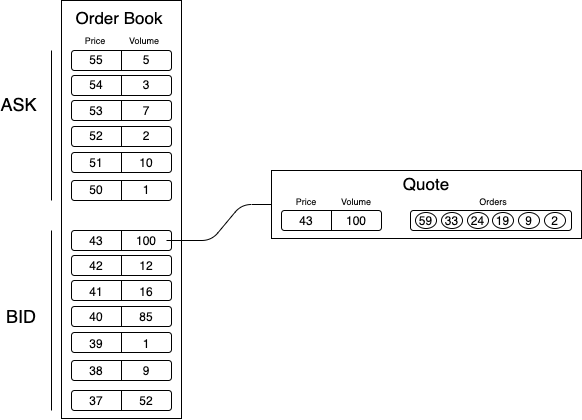
\includegraphics[width=450pt]{images/order_book_schema.png}
\end{center}

\newpage

В какой-то момент приходит заявка на покупку (продажу), которая по цене пересекает противоположное направление продажи (покупки). То есть находятся такие уже стоящие в стакане другие заявки на продажу (покупку), цена которых больше (меньше), и с ними можно организовать сделку. Заявка на покупку (продажу), спровоцировавшая такую сделку называется \textbf{активной}, а заявка на продажу (покупку), уже стоящая в стакане, называется \textbf{пассивной}. Выполнение этой логики обеспечивается \textbf{торговым движком}.


\begin{center}
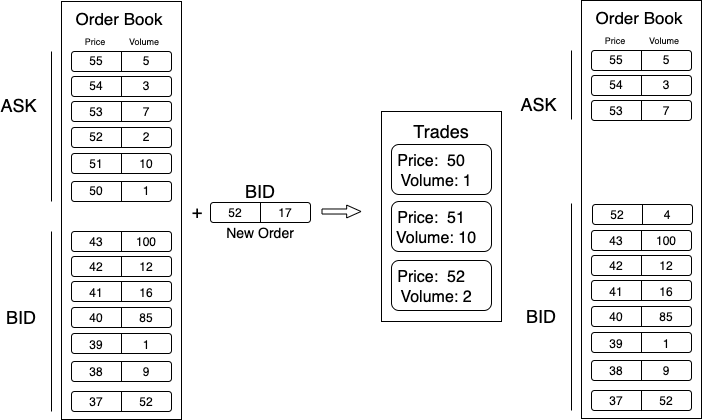
\includegraphics[width=450pt]{images/trade_schema.png}
\end{center}

Таким образом, участники торгов наглядно видят, сколько объема и по какой цене они могут купить или продать прямо сейчас активной заявкой, либо на какую цену они могут отправить пассивную заявку, чтобы ждать сделки в будущем.

\pagebreak
	%% Cильный и слабый пределы
		\section{Реализация биржи}
\subsection{Общая архитектура}
Поговорим теперь о реализации биржевой инфраструктуры. Нашей целью будет написать главные компоненты биржи и обеспечить их совместную работу.
Рассмотрим внутреннюю архитектуру типичной биржи. В качестве примера возьмем одну из самых крупных и известных - Чикагская биржа \textbf{CME} [1.2]

\begin{center}
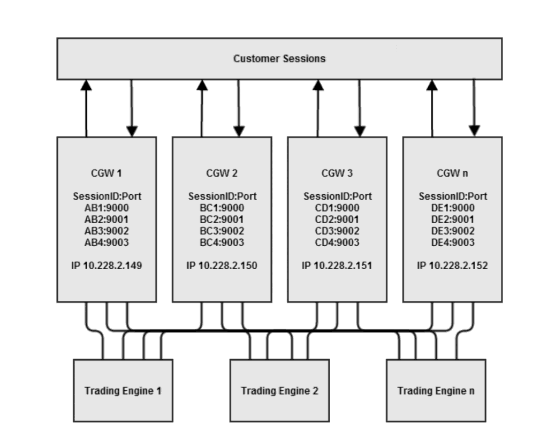
\includegraphics[width=400pt]{images/cme_schema.png}
\end{center}

Как можно видеть, главными компонентами биржи являются уже упомянутые выше торговые движки (Trading Engines в терминологии книги [1.2]). Посредником между ними и клиентами на этой схеме являются порты. Однако в реальности порты не только обеспечивают канал связи с клиентом, принимая его запросы (как это обычно принято подразумевать под термином "порт"), но и фильтруют их, предобрабатывают и распределяют очередь запросов, которую обрабатывает нужный торговый движок. Таким образом, более широкое и применимое определение этой сущности - \textbf{Connection Manager}.

В рамках этой работы будет рассмотрена упрощенная схема с одним торговым движком:

\begin{center}
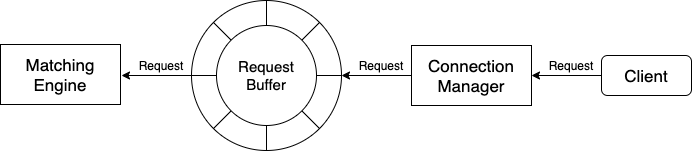
\includegraphics[width=400pt]{images/exchange_schema.png}
\end{center}


\textbf{Request Buffer} - это буффер запросов, куда они кладутся после поступления. Он будет асинхронно освобождаться торговым движком. Это один из ключевых компонентов с точки зрения нагрузоустойчивости: при его переполнении торги останавливаются до тех пор, пока все запросы не будут выполнены. Задача биржи устроить торги и инфраструктуру таким образом, чтобы этого не происходило.

\subsection{Backend}

Для написания бекенд части, я выбрал язык программирования \textbf{С++}. Он является низкоуровневым, высокопроизводительным и отказоустойчивым при правильной разработке. Кроме того, C++ в целом является стандартом разработки нагруженных компонент в финансовой индустрии.

Репозиторий с кодом открыт и находится по адресу

\begin{center} \url{https://github.com/evgenstf/market_load_prediction} \end{center}

При разработке я старался уделять большое внимания чистоте кода [3.1], правильным паттернам, тестам [3.2]  и общей логике[3.3].

Ниже представлена итоговая архитектура биржи, которая у меня получилась:


\begin{center}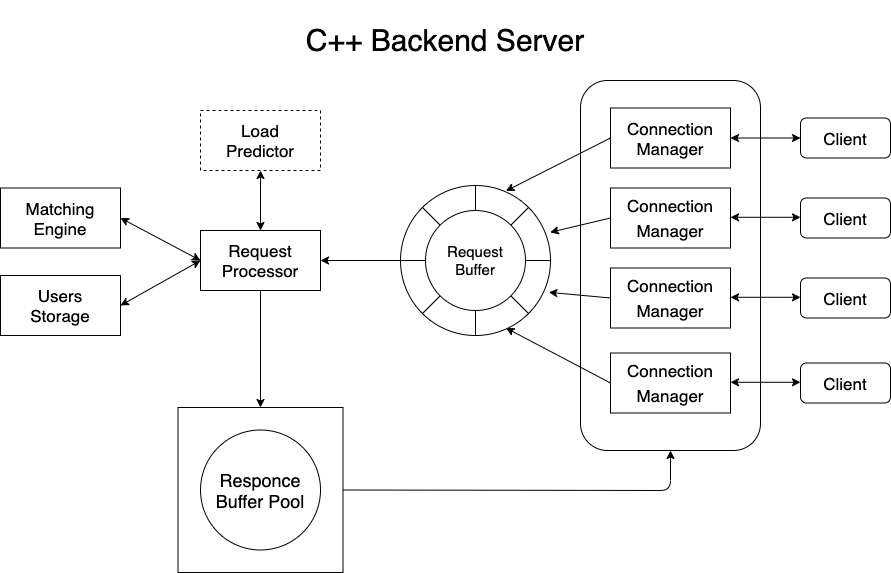
\includegraphics[width=450pt]{images/backend_schema.png}\end{center}

В ней присутствуют следующие основные компоненты:

\begin{itemize}
    \item \textbf{Connection Manager} - поддерживает соединение с клиентом по протоколу TCP и передает его запросы в \textbf{Request Buffer}.
    \item \textbf{Request Buffer} - асинхронное хранилище запросов.
    \item \textbf{Request Processor} - компонент, который достает запросы из \textbf{Request Buffer} и в зависимости от необходимой логики отправляет нужные команды в \textbf{Matching Engine} и. \textbf{User Storage}. После обработки запроса, отчет отправляется обратно в \textbf{Connection Manger} через \textbf{Response Pool}, который затем отправляется клиенту
    \item \textbf{User Storage} - сущность, хранящая личную информацию о клиентах: баланс, торговую историю, текущие заявки в биржевом стакане.
    \item \textbf{Matching Engine} - как уже было упомянуто, хранит биржевой стакан и обеспечивает логику сведения заявок в сделки.
    \item \textbf{Load Predictor} - компонент, предсказывающий нагрузку. О нем подробнее во второй части.
\end{itemize}


\newpage

\subsection{Frontend}

Для создания веб-интерфейса я использовал фреймворк под названием Django [3.4]. Это простое общеиспользуемое решение, которое легко применимо в данном случае.

Внутри содержится система изолированных каналов на основе Redis Server [3.5]. Это необходимо для того, чтобы поддерживать уникальное соединение с каждым пользователем по Websocket [3.6] (например, для отправки отчетов о сделках клиента) и отправлять пачку сообщений на группу пользователей, объединенных одним каналом (например, обновления стакана).

Фронтенд и бекенд серверы находятся на одной физической машине под управлением Ubuntu Server и общаются друг с другом посредством протокола TCP.

\begin{center}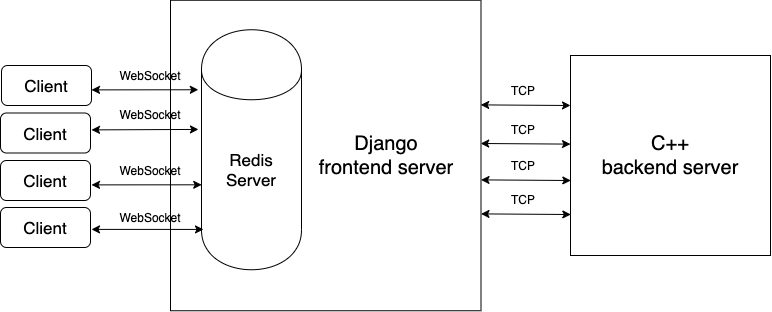
\includegraphics[width=450pt]{images/frontend_schema.png}\end{center}

\newpage
Веб интерфейс получился довольно лаконичным, и, в то же время, функциональным:

\begin{center}
    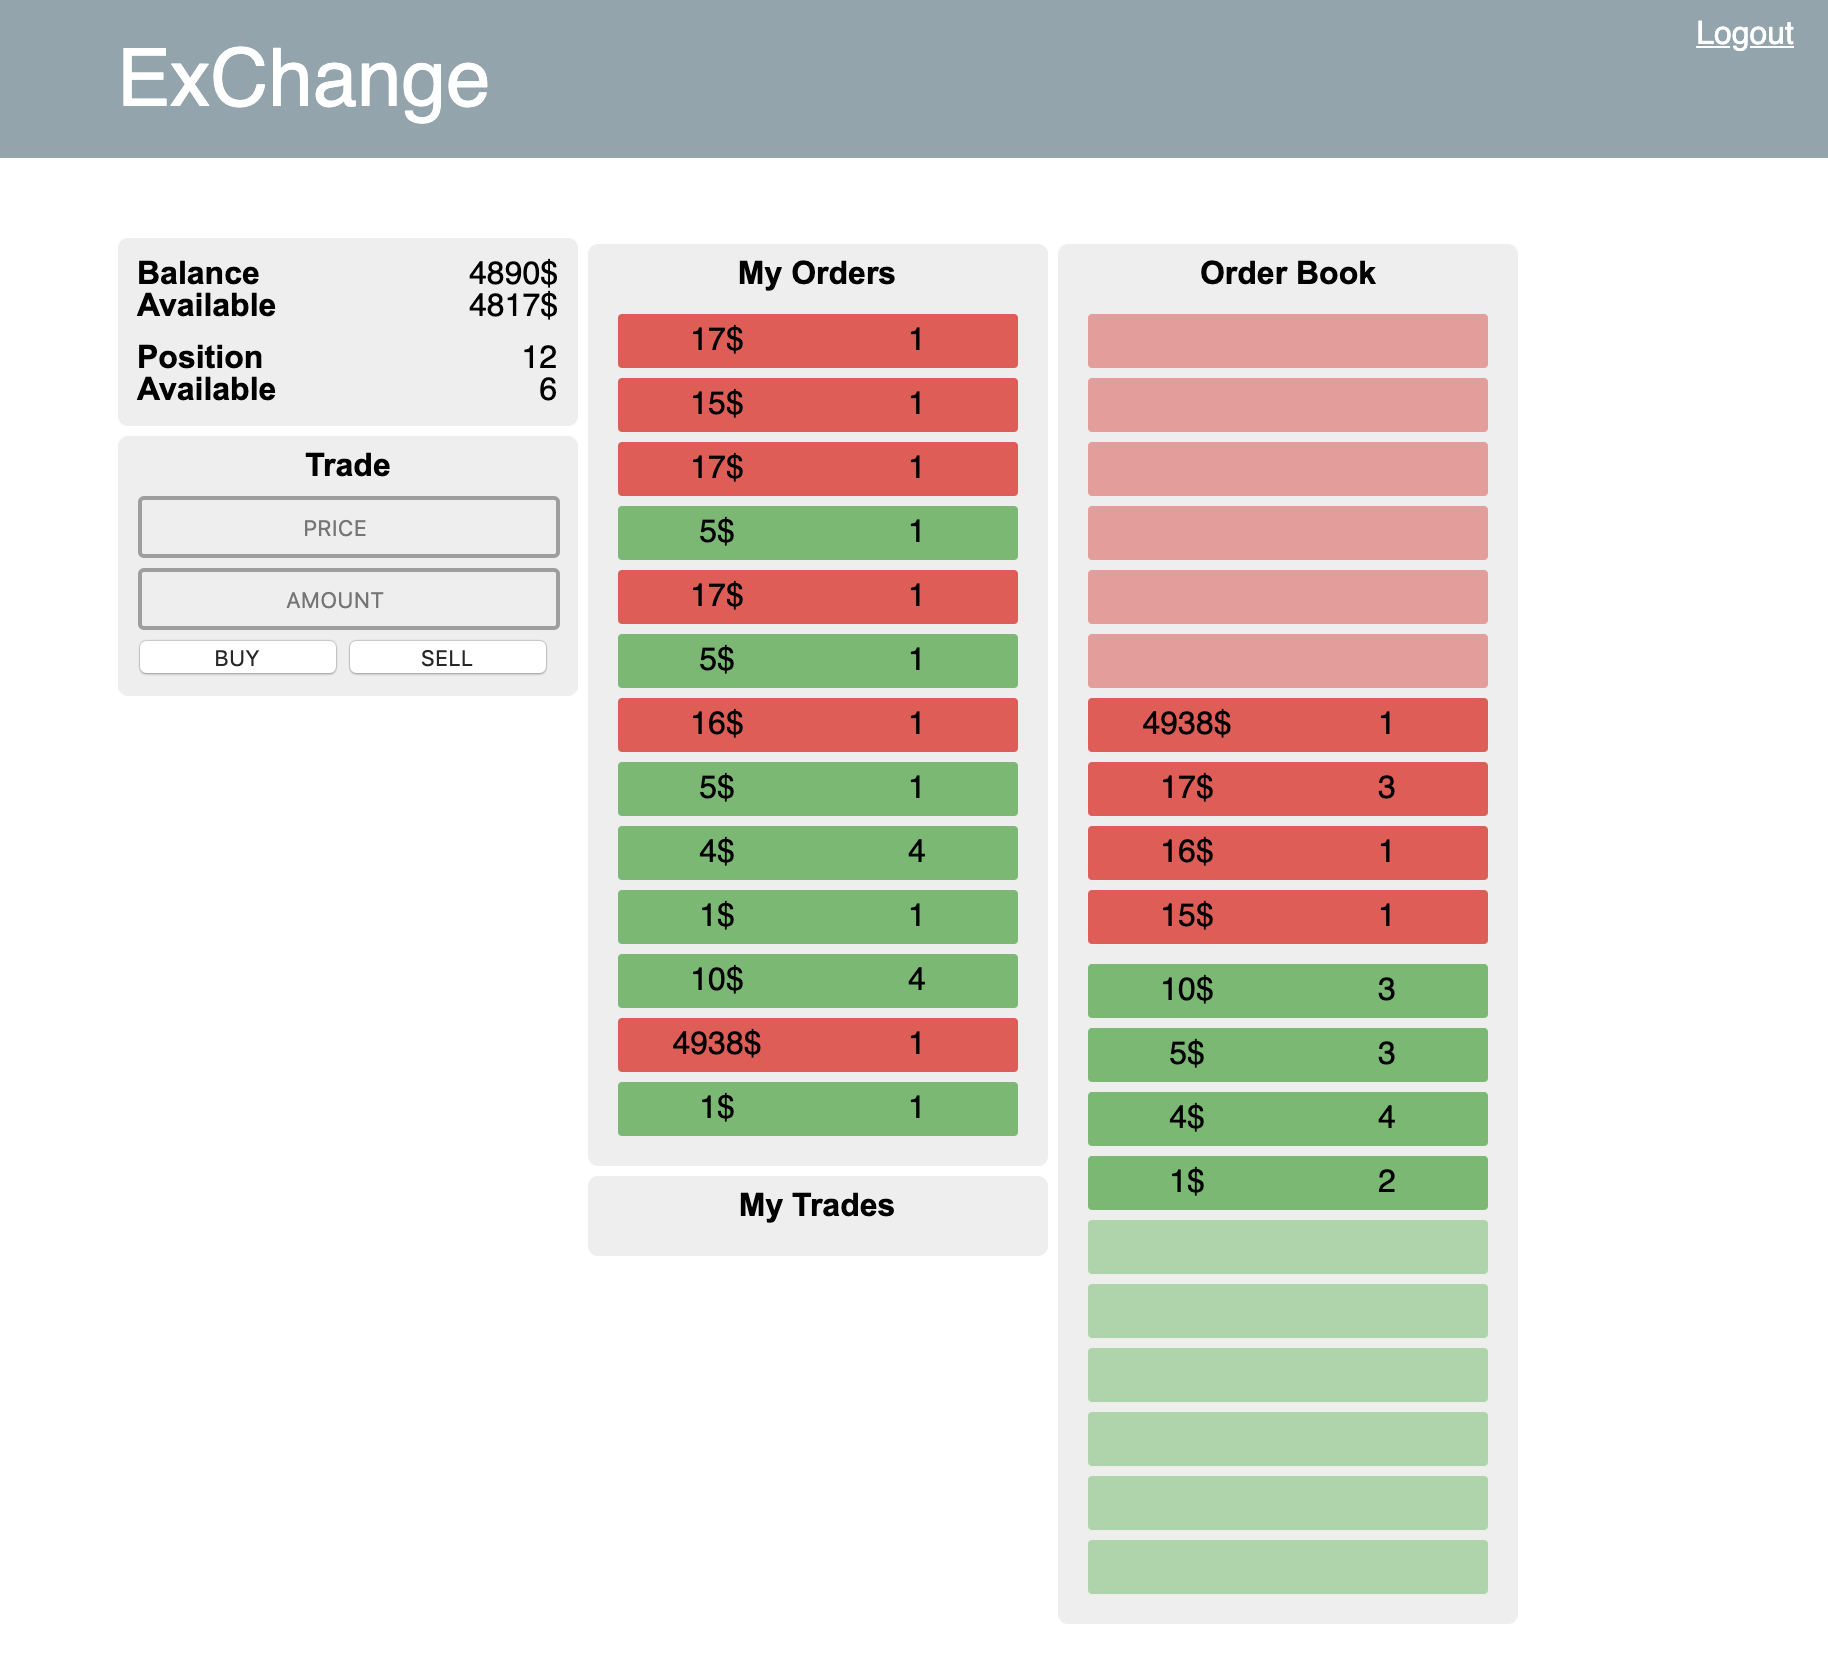
\includegraphics[width=450pt]{images/interface_screenshot.png}
\end{center}

Как можно видеть, на нем присутствуют: секция для отправки заявки, сделки пользователя, заявки пользователя, стоящие в стакане и, собственно, сам биржевой стакан.

\newpage
\subsection{Нагрузочное тестирование }

Для нагрузочного тестирования и проверки предсказывающих моделей был разработан CLI (Command line interface) инструмент, который эмулирует участника торгов и посылает заявки с конфигурируемым разбросом цен, объемом и частотой.

Я запустил его с несколькими значениями частоты отправки запросов и засек время, через которое буффер запросов переполняется. В таблице ниже представлены эти значения:


\begin{center}
\begin{tabular}{ c c }
 Requests per sec & Time till overflow in sec \\ 
 <1000 & $+\infty$\\
 1500-2500 & 950 \\
 2500-3500 & 300 \\
 3500-10000 & 100 \\
\end{tabular}
\end{center}

Отсюда можно сказать, что опытным путем была установлена производительность написанной биржи: 1000-1500 запросов в секунду (один запрос занимает от 600 до 1000 микросекунд).


\newpage
	%% Cильный и слабый пределы
		\section{Предсказание волатильности}
После реализации биржи можно, наконец, перейти к исследованию по предсказанию динамики торговой нагрузки на нее.

Прежде всего необходимо формализовать само понятие "биржевая нагрузка", чтобы понять какую величину мы хотим предсказывать. В рамках этой работы мы сделаем это следующим образом:

\begin{quote}
\textbf{Биржевая нагрузка} - количество входящих заявок, поступающих за одну секунду.
\end{quote}

От ее величины будет зависеть заполненность буффера, о которой было упомянуто в пункте про нагрузочное тестирование.


\subsection{Данные}

Для анализа и обучения были выбраны данные торгов криптовалюты Bitcoin.
Криптовалюты более всего удобны для исследований, прежде всего потому что эта сфера финансов одна из самых открытых и доступных: 
торговую историю можно без дополнительных вложений получить практически от любой криптовалютной биржи. Кроме того, эти данные имеют удобный формат: биржевые стаканы имеют достаточную глубину в 10-20 котировок, а временные моменты расписаны с точностью до миллисекунд.



\subsection{Предсказывающие модели}


Ниже приведены наложенные графики двух величин: ценa и количество запров за некоторый промежуток времени.

\begin{center}
    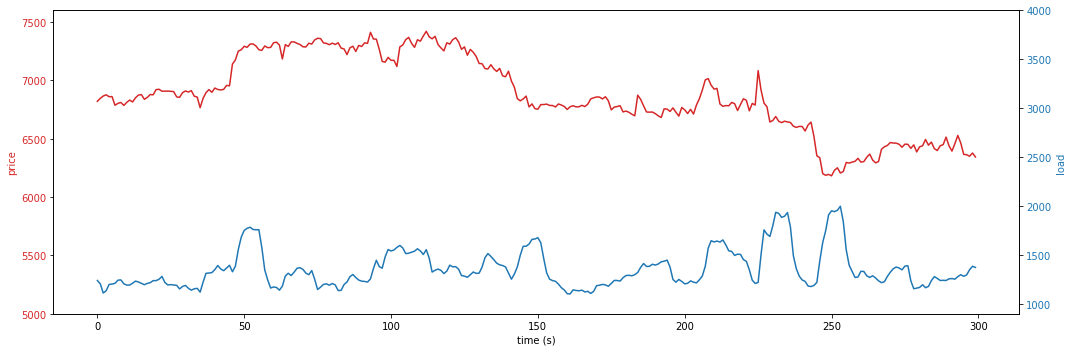
\includegraphics[width=450pt]{images/graph_price_load.png}
\end{center}

Можно видеть, что количество запросов коррелирует с динамикой цены: после резких скачков цены происходит также резкое повышение количества запросов, обусловленное стремлением рынка к корректировке. Это вполне очевидная зависимость, поэтому мы действительно можем подразумевать под волатильностью как скорость изменения цены, так и величину биржевой нагрузки.

\newpage

Посмотрим также на график наполненности буффера запросов, наложенный на график количества запросов:
\begin{center}
    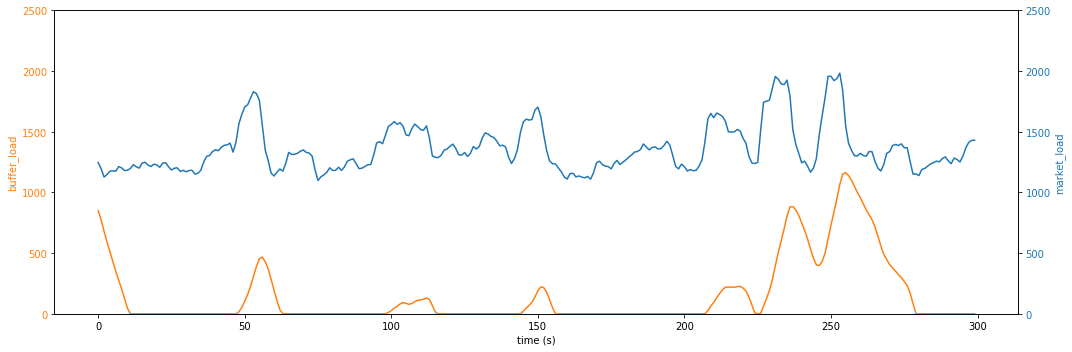
\includegraphics[width=450pt]{images/graph_buffer_load.png}
\end{center}

Видно, что при достижении количества запросов от клиентов некоторого порогового значения около 1500 запросов в секунду, наполненность буффера начинает расти из-за того, что торговый движок не успевает обрабатывать заявки.

\subsubsection{Статистическая модель}

По графикам выше можно предположить, что для предсказания нагрузки достаточно использовать простую статистическую модель, основанную, например, на скользящем среднем.

И действительно, поскольку резкое изменение цены является надежным сигналом к последующей реакции рынка, мы можем отслеживать ценовую динамику за последние секунды
и на основании этого делать прогнозы по увеличению количества поступающих запросов.

Для этого будем использовать модель из пакета

\textbf{statsmodels.tsa.arima\_model} под названием \textbf{ARMA}, являющуюся обобщением авторегрессии и скользащего среднего [2.1], [2.2].

Предсказание будет производиться в два этапа:
\begin{itemize}
    \item 1. Преобразуем временной ряд цен во временной ряд разниц цен
    \item 2. По временному ряду разниц цен будем предсказывать биржевую нагрузку с помощью ARMA
\end{itemize}

Полученный временной ряд с разницами цен, наложенный на график нагруженности:

\begin{center}
    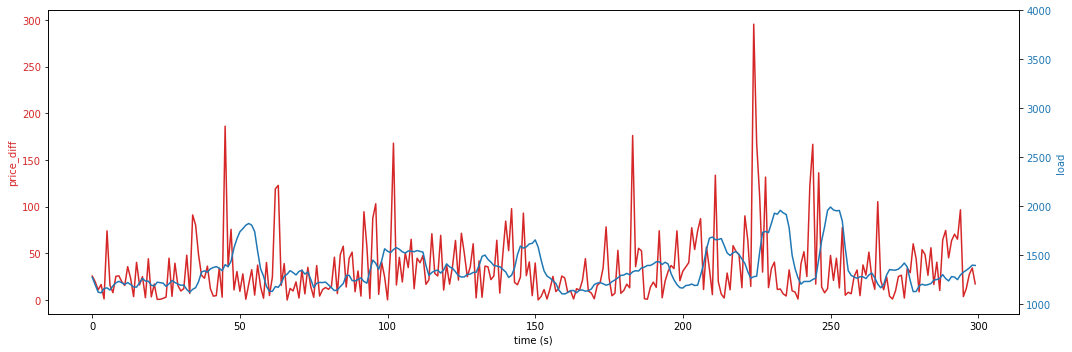
\includegraphics[width=450pt]{images/graph_diff_load.png}
\end{center}

Видно, что повышению нагрузки предшествуют резкие скачки цены. Для удобства можно оставить только те значения разниц цен, которые больше некоторого порогового значения:


\begin{center}
    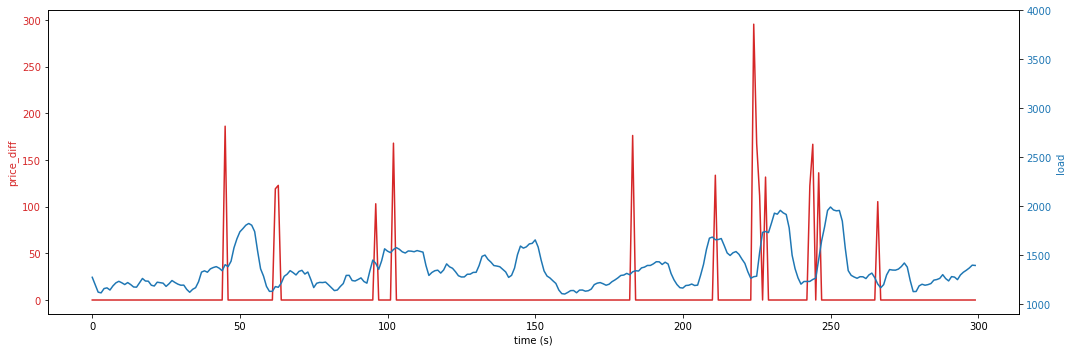
\includegraphics[width=450pt]{images/graph_diff_load_2.png}
\end{center}

Попробуем теперь предсказывать разницу цен с помощью ARMA. График такого предсказания:


\begin{center}
    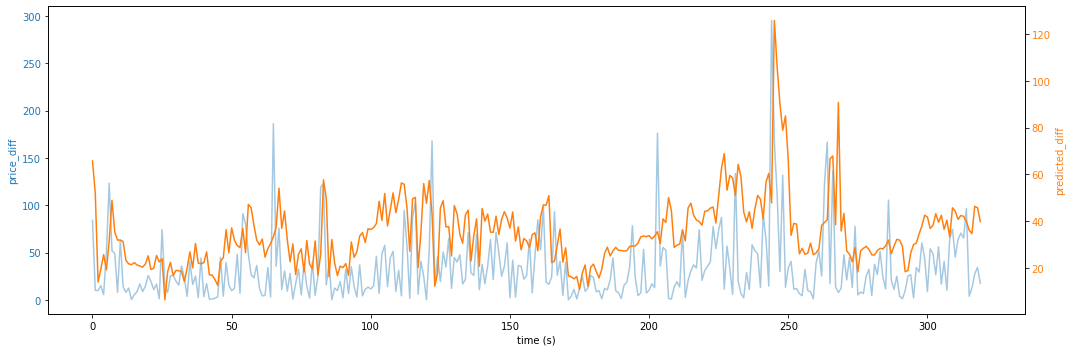
\includegraphics[width=450pt]{images/graph_arma_prediction.png}
\end{center}

Видно, что на больших пиках (в районе 200 сек) предсказание довольно успешно. Однако средние повышения остаются не предсказанными.
\newpage
\subsubsection{Рекуррентные сети}

Одними из самых распространенных моделей для предсказания временных рядов в финансах традиционно считаются рекуррентные сети. Вкратце разберем, как они работают [2.3], [2.4].

Обычная нейронная сеть состоит из набора слоев с нейронами, последовательно соединенными друг с другом. На вход поступает некоторый набор значений, он проходит через все слои и на выходе выдается некоторая величина в качестве ответа.


\begin{center}
    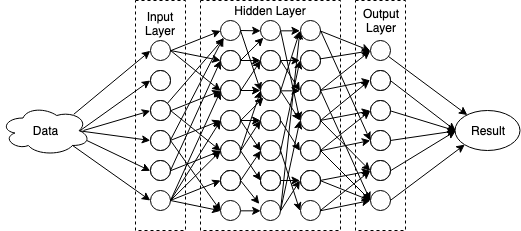
\includegraphics[width=450pt]{images/network_schema.png}
\end{center}

В рекуррентной же сети добавляется еще одно входное значение - предсказание модели на предыдущем шаге:

\begin{center}
    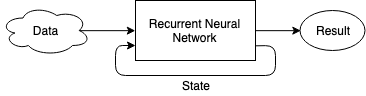
\includegraphics[width=300pt]{images/network_schema_2.png}
\end{center}
\newpage

Это можно для удобства раскрыть как несколько сетей, каждая из которых передает значение предсказания в следующую:

\begin{center}
    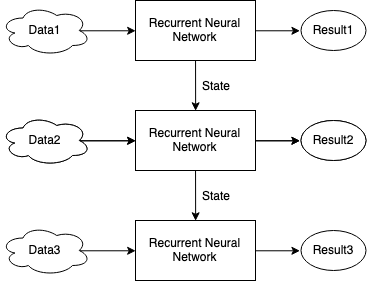
\includegraphics[width=300pt]{images/network_schema_3.png}
\end{center}

Такая архитектура позволяет хранить некоторый контекст, в котором происходит предсказание. На практие это это дает значительное улучшение в результатах, и используется, например, в предсказании погоды [2.5].
\newpage
Я использовал простую реализацию \textbf{RNN} из пакета \textbf{keras}.

Ниже приведена полная конфигурация сети:
\begin{small}
\begin{verbatim}
    Model: "sequential_3"
______________________________________________
Layer (type)    Output Shape   Param #   
==============================================
simple_rnn_3 (SimpleRNN) (None, 32)        1184      
______________________________________________
dense_5 (Dense)          (None, 8)         264       
______________________________________________
dense_6 (Dense)          (None, 1)         9         
==============================================
Total params: 1,457
Trainable params: 1,457
Non-trainable params: 0
______________________________________________
\end{verbatim}
\end{small}

Полученные в результате работы предсказания:

\begin{center}
    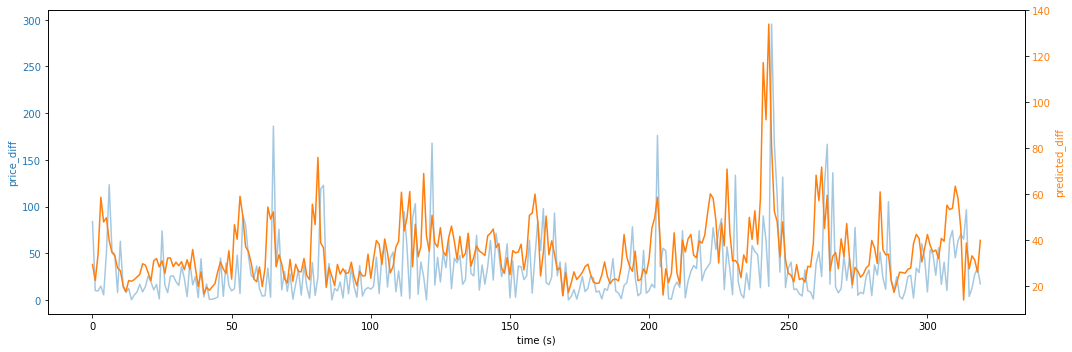
\includegraphics[width=450pt]{images/graph_rnn_prediction.png}
\end{center}

Видно, что предсказания стали точнее: пики изменения цен, предшествующие повышению нагрузки, стали отчетливее и соответствуют тому, что происходило в реальности.
\newpage

\subsection{Сравнительное тестирование}

В качестве критерия качества предсказаний полученных моделей я выбрал способность давать правильные сигналы-предупреждения о надвигающейся активности.

Для этого на исходных данных я разметил моменты, когда поступающие запросы превосходят производительность торгового движка (1500 запросов в секунду).

Корректным сигналом считается превышение порогового значения $P$ в предсказании от модели. Я провел несколько экспериментов с различными константами, результаты F-меры приведены в таблице ниже.


\begin{center}
\begin{tabular}{ c c c }
 P & ARMA & RNN \\ 
40 & 0.60 & 0.84 \\
50 & 0.71 & 0.97 \\
60 & 0.54 & 0.98 \\
70 & 0.54 & 0.77 \\
80 & 0.54 & 0.66 \\
90 & 0.54 & 0.60 \\
\end{tabular}
\end{center}

Таким образом, наилучшие значения предсказания достигаются при $P = 50$.

\newpage	%% Cильный и слабый пределы
		\section{Заключение}

В качестве итога проделанной работы предлагаю еще раз закрепить то, к чему мы пришли в ходе нее.

Была реализованна и протестированная полноценная биржа, предназначенная для высокочастотной торговли. В ходе испытаний было установлено, что ее производительность достаточна для обработки запросов с реальных торгов.

Было проведено исследование нескольких моделей по предсказанию увеличения торговой нагрузки. Результаты соответствуют ожиданиям.
	%% Cильный и слабый пределы
		\newpage
\section{Список литературы}
\subsection{Финансы}
\begin{itemize}
\item [1.1] William T. Bagley, Gary L. Seevers, “Glossary of trade terms” in Glossary of Some Terms Commonly Used In The Futures Trading Industry. New York, USA. 1978.
\item [1.2] Xin Guo, Tze Leung Lai, Howard Shek,
Exchange infrastructure” in Quantitative Trading: Algorithms, Analytics, Data, Models, Optimization. 6000 Broken Sound Parkway NW, Suite 300. 2017. ISBN-13: 978-1-4987- 0648-3
\end{itemize}
\subsection{Предсказывающие модели}
\begin{itemize}
\item [2.1] Time Series Analysis for Financial Data IV— ARMA Models, 2017, Medium
\item [2.2] Alvin C. Rencher, G. Vruce Schaalje “SIMPLE LINEAR REGRESSION MODEL” in Linear Models In Statistics, Hoboken, New Jersey, 2008. ISBN-13: 978-0-471-75498-5
\item [2.3] Е. А. Казаков, Выявление токсичного контента на портале для обмена знаниями Quora, 2019
\item [2.4] Christopher Olah, Understanding LSTM Networks, 2014
\item [2.5] Saroj Kr. Biswas, Nidul Sinha, Biswajit Purkayastha, Leniency Marbaniang, Weather prediction by recurrent neural network dynamics, 2014, DOI: 10.1504/IJIEI.2014.066208
\end{itemize}
\subsection{Программирование}
\begin{itemize}
\item [3.1] Robert Martin Clean Code, 2008, ISBN-10: 9780136083238
\item [3.2] Kent Beck Test-Driven Development, ISBN-13: 978-0321146533
\item [3.3] Scott Chacon, Ben Straub, Pro Git, Mountain View, CA 94042, USA. 2020
\item [3.4] Django Software Foundation, Django Documentation, Release 3.0.7.dev
\item [3.5] Karl Seguin, The little Redis book
\item [3.6] Andrew Lombardi, WebSocket: Lightweight Client-Server Communications, ISBN-13: 978-1449369279

\end{itemize}	%% Cильный и слабый пределы
		\newpage
\section{Приложениe}

Ниже приведены ссылки на репозиторий по компонентам, упомянутым в работе.

\subsection{Backend}

\begin{itemize}
    \item \textbf{Connection Manager} - \url{https://github.com/evgenstf/market_load_prediction/blob/master/backend/connection_manager/connection_manager.h}
    \item \textbf{Matching Engine} - \url{https://github.com/evgenstf/market_load_prediction/blob/master/backend/matching_engine/matching_engine.h}
    \item \textbf{Request Buffer} - \url{https://github.com/evgenstf/market_load_prediction/blob/master/backend/entities/ring_buffer/ring_buffer.h}
    \item \textbf{User Storage} - \url{https://github.com/evgenstf/market_load_prediction/blob/master/backend/user_storage/user_storage.h}
    \item \textbf{Market Maker} - \url{https://github.com/evgenstf/market_load_prediction/blob/master/load_prediction/market_maker.py}

\end{itemize}
    
\subsection{Frontend}

\begin{itemize}
    \item \textbf{Common} - \url{https://github.com/evgenstf/market_load_prediction/tree/master/frontend}
    \item \textbf{Interface} - \url{https://github.com/evgenstf/market_load_prediction/blob/master/frontend/templates/index.html}
    \item \textbf{Server} - \url{https://github.com/evgenstf/market_load_prediction/blob/master/frontend/chat/consumers.py}
\end{itemize}

\subsection{Prediction Research}
\url{https://github.com/evgenstf/market_load_prediction/blob/master/load_prediction/research.ipynb}	%% Cильный и слабый пределы
		
\end{document}

%%
%%
%%
